\documentclass[12pt]{article}
\usepackage{pgf, tikz}
\usepackage{amsmath, amsfonts, amssymb, graphicx}
\usepackage{subfig}
\usepackage{float}
\usepackage[utf8]{inputenc}
\usepackage[spanish]{babel}
\usepackage{amsthm}

\setlength{\textheight}{23cm} \setlength{\evensidemargin}{0cm}
\setlength{\oddsidemargin}{-.5cm} \setlength{\topmargin}{-3cm}
\setlength{\textwidth}{17.5cm} \setlength{\parskip}{.2cm}


%opening

\begin{document}
	\begin{picture}(80, 80)
	\put(170,0){\hbox{
\includegraphics[scale=0.6]{cimat_logo.png}}}
	\end{picture}
	
	\begin{center}
		\begin{huge}
			Centro de Investigación en Matemáticas, A.C.
		\end{huge}
	\end{center}

	\begin{center}
		\begin{large}
			Descripción tarea 4: Ejercicio 2 - Métodos numéricos
		\end{large}
	\end{center}
	
	\begin{center}
		\textbf{Erick Salvador Alvarez Valencia}
	\end{center}

	\begin{center}
		23 de Septiembre de 2017
	\end{center}



%\maketitle

%\tableofcontents

\section{Descripción}
El presenta programa resuelve un sistema de ecuaciones tipo $Ax = b$ donde $A$ es una matriz tridiagonal, y dicho sistema se generó al intentar resolver la ecuación de Poisson en una dimensión.\\
La matríz $A$ es generada de acuerdo a como lo dice la tarea, el sistema calcula el tamaño de paso, los vectores $x_i$ y $b$, y aplica la resolución usando el método del ejercicio 1. El programa generará un archivo de texto, la matríz de los resultados generados por el algoritmo.

\section{Compilación y ejecución}
\textbf{Para compilar:} En la carpeta encontraremos los archivos $.c$ y $.h$ con los que se podrá compilar el ejecutable. De la misma forma, en conjunto con los archivos anteriores, también podremos encontrar un Makefile para, en caso de encontrarse en linux, compilar de manera sencilla.

\begin{enumerate}
	\item \textbf{Compilar usando Makefile:} En la terminal, nos colocamos en el directorio donde se encuentre el programa, y ejecutamos el comando $make$, automáticamente se realizará la compilación y se generará el ejecutable.\\
	\item \textbf{Compilar directamente:} De la misma forma, podemos compilar directamente usando los siguientes comandos (en terminal):\\
	\begin{itemize}
		\item gcc -c main.c
		\item gcc -c memo.c
		\item gcc -c matriztridiagonal.c
		\item gcc -c reader.c
		\item gcc -o main main.o memo.o matriztridiagonal.o reader.o -lm
	\end{itemize}
\end{enumerate}

\textbf{Para ejecutar:} Únicamente debemos de usar el comando $./main$ para ejecutar el programa en consola.\\
El programa recibe un argumento, un entero, el número de particiones que se realizarán. A continuación se mostrará un ejemplo de cómo ejecutar el programa:\\

$./main\ 10$

\section{Ejemplo de ejecución}

A continuación se mostrarán ejemplos de ejecución del programa con 10 y 100 particiones:\\

\begin{figure}[H]
	\centering
	\subfloat[][Figura 1. Resultado de la ejecución del programa con 10 particiones.]{
		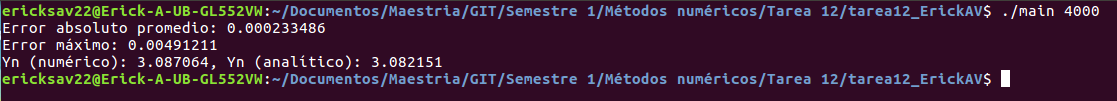
\includegraphics[scale=0.3]{E2.png}
	}\hfill
\end{figure}

\begin{figure}[H]
	\centering
	\subfloat[][Figura 1. Resultado de la ejecución del programa con 100 particiones.]{
		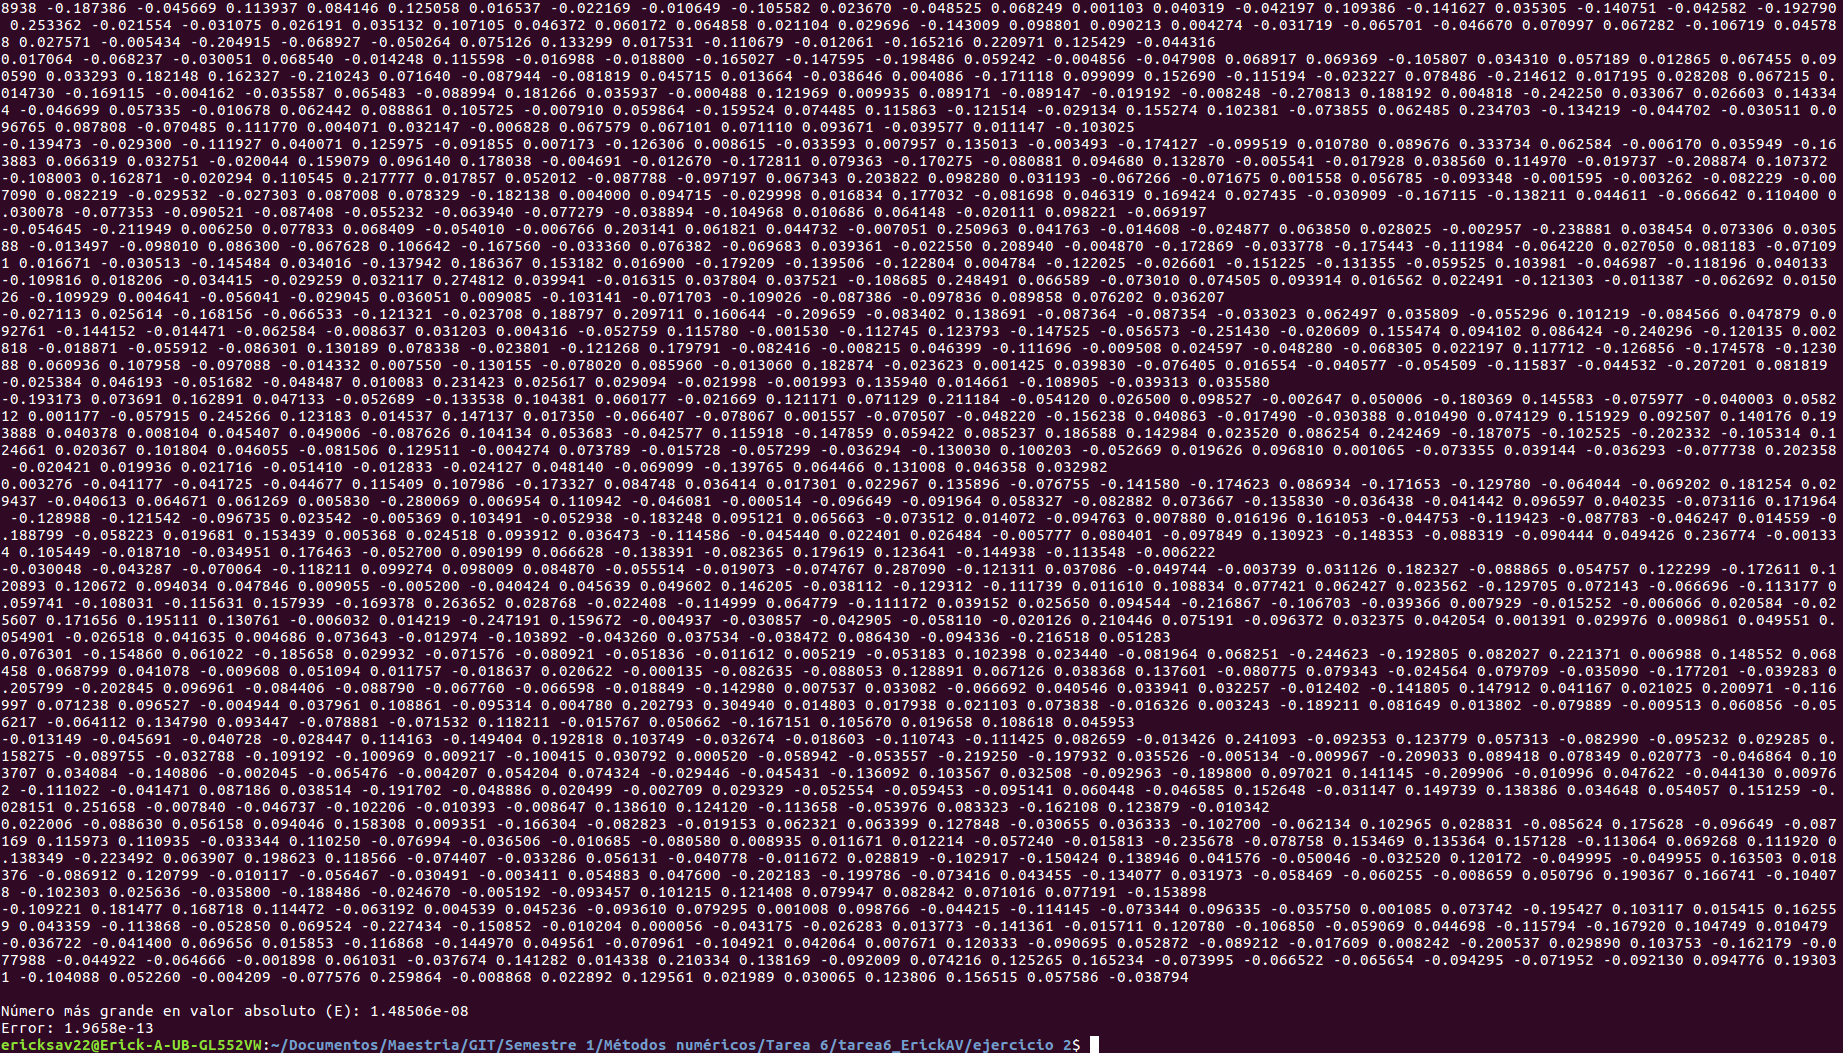
\includegraphics[scale=0.2]{E3.png}
	}\hfill
\end{figure}

\end{document}
